\documentclass[english, aspectratio=169]{beamer}
% english is for the language used in standard texts (figures, tables etc)
% aspectratio of 16:9 or set it for more old school to 4:3 (without the ':')

% ---------------------------------------------------------------------------- %
% Load base preamble
% ---------------------------------------------------------------------------- %
\usepackage{import}
\subimport{../preamble/}{beamer.tex}

% ---------------------------------------------------------------------------- %
% Local settings
% ---------------------------------------------------------------------------- %
% https://tex.stackexchange.com/a/20613
\newcommand\hcancel[2][black]{\setbox0=\hbox{$#2$}%
  \rlap{\raisebox{.35\ht0}{\textcolor{#1}{\rule{\wd0}{1pt}}}}#2}

\newcommand{\B}[0]{\ensuremath{\mathbb{B}}}
\newcommand{\pow}[0]{\ensuremath{\mathcal{P}}}

\newcommand{\sort}[0]{\text{sort}}

\newcommand{\triple}[3]{\ensuremath{(#1, #2, #3)}}
\renewcommand{\arc}[3]{\ensuremath{#1 \xrightarrow{_{#2}} #3}}

\tikzstyle{plot_instance}=[color=gray, mark=none, line width=0.7pt, densely dotted]
\tikzstyle{plot_adiar}=[color=blue, mark=o, mark size=1.5pt, line width=1pt, solid]
\tikzstyle{plot_cudd}=[color=red, mark=diamond, mark size=1.5pt, line width=1pt, solid]

% Horizontal legends: https://tex.stackexchange.com/a/101578
% argument #1: any options
\makeatletter
\newenvironment{customlegend}[1][]{%
    \begingroup
    % inits/clears the lists (which might be populated from previous
    % axes):
    \pgfplots@init@cleared@structures
    \pgfplotsset{#1}%
}{%
    % draws the legend:
    \pgfplots@createlegend
    \endgroup
}%

% makes \addlegendimage available (typically only available within an
% axis environment):
\def\addlegendimage{\pgfplots@addlegendimage}
\makeatother

% ------------------------------------------------------------------------------
% TITLEPAGE
% ------------------------------------------------------------------------------
\title{
  Adiar 1.1 : Zero-suppressed Decision Diagrams\\\hspace{80pt}in External Memory
}

\author{{\bf Steffan Christ S{\o}lvsten} and Jaco van de Pol}

\institute{
\includegraphics[width=0.2\linewidth]{../external/aulogo_uk_var2_black.eps}}

\date{$18^{\text{th}}$ of May, 2023}

\begin{document}

\titleframe

\blankframe

\begin{frame}
  \begin{figure}
    \centering

    \begin{tikzpicture}
      % Numbers from:
      % - Intel® 64 and IA-32 Architectures Optimization Reference Manual
      %   + Cache: Table 2-7/2-14
      %   + RAM:   3.6.10 Locality Enhancement
      % - www.lighterra.com/papers/modernmicroprocessors/
      %   + SSD: Extrapolation from the 2.000.000 to fit Intel's Manual.
      % - imada.sdu.dk/u/rolf/Edu/DM79/E04/Slides/IOModel.pdf
      %   + HDD: Extrapolation from the 2.000.000 to fit Intel's Manual.

      % ALU
      \node[
        draw,
        trapezium,
        shape border rotate=180,
        text width=0.8cm,
        align=center,
      ] at (0,0) (cpu) {CPU};

      % Cache
      \draw[draw=gray, rounded corners=3pt, densely dotted, line width = 0.6pt]
      (-1.3,2.3) rectangle ++(2.6,-1.6);

      \node[
        draw,
        rectangle,
        text width=0.3cm,
        align=center,
      ] at (0,1) (l1) {\tiny L1};

      \node[
      draw,
      rectangle,
      text width=0.8cm,
      align=center,
      ] at (0,1.45) (l2) {\tiny L2};

      \node[
        draw,
        rectangle,
        text width=2cm,
        align=center,
      ] at (0,1.95) (l3) {\footnotesize L3};

      \path[->]
        (cpu) edge[bend left=25] (l1)
        (l1) edge[bend left=25] (cpu)
      ;
      \onslide<3->{\node at (2.8,0.5) {$\sim$ 4 -- 50 CPU Cycles};}

      % Main memory
      \node[
        draw,
        rectangle,
        text width=4cm,
        align=center,
      ] at (0,3.5) (ram) {RAM};

      \path[->]
        (l3) edge[bend left=40] (ram)
        (ram) edge[bend left=40] (l3)
      ;
      \onslide<3->{\node at (2.6,2.7) {$\sim$ 200 CPU Cycles};}

      % Disk
      \only<2-3> {
        \node[
          draw,
          cylinder,
          minimum width=8cm,
          aspect=0.3,
          align=center,
          shape border rotate=90
        ] at (0,5.5) (disk) {SSD};
      }
      \onslide<4> {
        \node[
        draw,
        cylinder,
        minimum width=12cm,
        aspect=0.26,
        align=center,
        shape border rotate=90
        ] at (0,5.5) (disk) {HDD};
      }

      \only<2->{
        \path[->]
          (disk) edge[bend left=40] (ram)
          (ram)  edge[bend left=40] (disk)
        ;
      }
      \only<3>{\node at (3,4.5) {$\sim$ 200.000+ CPU Cycles};}
      \onslide<4->{\node at (3.25,4.5) {$\sim$ 20.000.000+ CPU Cycles};}
    \end{tikzpicture}
  \end{figure}
\end{frame}

\begin{frame}[plain,noframenumbering]{}
  \begin{center}
    {\LARGE
      \only<1>{%
        Binary%
      }%
      \only<2>{%
        {\textbf{Multi-terminal}}%
      }%
      \only<3>{%
        {\textbf{Quantum Multi-valued}}%
      }%
      \only<4>{%
        {\textbf{Zero-suppressed}}%
      }%

      Decision Diagrams
    }
  \end{center}
\end{frame}

\begin{frame}
  \begin{figure}
    \centering

    \begin{tikzpicture}[every node/.style={transform shape}]
      % nodes
      \node[shape = circle, draw = black]
      (0) {$x_0$};

      \node[shape = circle, draw = black, below left=1.4cm and .5cm of 0]
      (21) {$x_2$};

      \node[shape = circle, draw = black, below right=1.4cm and .5cm of 0]
      (22) {$x_2$};

      \node[shape = circle, draw = black, below right=0.4cm and .5cm of 21]
      (3) {$x_3$};

      % leafs
      \node[shape = rectangle, draw = black, below left=.4cm and .5cm of 3]
      (sink_F) {$0$};

      \node[shape = rectangle, draw = black, below right=.4cm and .5cm of 3]
      (sink_T) {$1$};

      % arcs
      \draw[->, dashed]
      (0)  edge (21)
      (21) edge (sink_F)
      (22) edge (3)
      (3)  edge (sink_F)
      ;

      \draw[->]
        (0)  edge (22)
        (21) edge (3)
        (22) edge (sink_T)
        (3)  edge (sink_T)
      ;

      % semantics
      \onslide<2>{
        \node[below right=0.1cm and 0.4cm of 0] {$x_0 = 1$};
        \node[below left=0.1cm and 0.4cm of 0]  {$x_0 = 0$};
      }
    \end{tikzpicture}
  \end{figure}
\end{frame}

\begin{frame}
  \begin{figure}
    \centering

    \begin{subfigure}[b]{0.32\linewidth}
      \centering

      \begin{tikzpicture}[every node/.style={transform shape}]
        \node[shape = circle, black, draw = black] (i) {$x_i$};
\node[shape = circle, draw = black, below=of i] (child) {};
\node[shape = circle, draw = black, above=of i] (parent) {};

% implication
\node[shape = circle, black,right=0.5cm of i] {$\implies$};

% after
\node[shape = circle, draw = black, right=2.5cm of child] (childafter) {};
\node[shape = circle, draw = black, right=2.5cm of parent] (parentafter) {};

\draw[->, dashed] (i) edge[bend right] (child);
\draw[->]
(i) edge[bend left] (child)
(parent) edge (i)
(parentafter) edge (childafter)
;

      \end{tikzpicture}

      \vspace{10pt}
      {\small {\bf BDD: } $f : \B^n \rightarrow \B$}
    \end{subfigure}
    \qquad\pause
    \begin{subfigure}[b]{0.32\linewidth}
      \centering

      \begin{tikzpicture}[every node/.style={transform shape}]
        \node[shape = circle, black, draw = black] (i) {$x_i$};
\node[shape = circle, draw = black, below left=1.2 and 0 of i] (child) {};
\node[shape = rectangle, draw = black, below right=1 and 0 of i] (terminal) {$0$};

\node[shape = circle, draw = black, above=of i] (parent) {};

% implication
\node[shape = circle, black,right=0.5cm of i] {$\implies$};

% after
\node[shape = circle, draw = black, right=2.4cm of child] (childafter) {};
\node[shape = circle, draw = black, right=2cm of parent] (parentafter) {};

\draw[->, dashed] (i) edge[bend right=5] (child);
\draw[->]
  (i) edge[bend left=5] (terminal)
  (parent) edge (i)
  (parentafter) edge (childafter)
;

      \end{tikzpicture}

      \vspace{10pt}
      {\small {\bf ZDD: } $A \subseteq \B^n$}
    \end{subfigure}
  \end{figure}
\end{frame}

\begin{frame}
  \Large

  \setvalue{type_color = orange}
  \setvalue{keyword_color = blue}
  \setvalue{other_color = black}

  \only<5> {
    \setvalue{type_color = orange!30!white}
    \setvalue{keyword_color = blue!30!white}
    \setvalue{other_color = black!30!white}
  }

  \texttt{%
    {\color{\getvalue{type_color}} bdd}
    {\color{\getvalue{other_color}} bdd\_apply(}%
    {\color{\getvalue{type_color}} bdd}
    {\color{\getvalue{other_color}} f,}
    {\color{\getvalue{type_color}} bdd}
    {\color{\getvalue{other_color}} g,}
    {\color{\getvalue{type_color}} bool\_op}
    {\color{\getvalue{other_color}} o)}
  } %
  \onslide<3-> {
    \texttt{{\color{\getvalue{other_color}} \{}}

    \qquad
    \texttt{{\color{\getvalue{keyword_color}} return}}
    \only<3>{\texttt{prod2(f, g, o, bdd\_strategy)}}%
    \only<4-5>{\texttt{%
        prod2%
        {\color{\getvalue{other_color}}<}%
        bdd\_policy%
        {\color{\getvalue{other_color}}>(f, g, o)}
      }}

    \texttt{{\color{\getvalue{other_color}} \}}}
  }

  \vspace{20pt}

  \onslide<2-> {
    \texttt{%
      {\color{\getvalue{type_color}} zdd}
      {\color{\getvalue{other_color}} zdd\_binop(}%
      {\color{\getvalue{type_color}} zdd}
      {\color{\getvalue{other_color}} A,}
      {\color{\getvalue{type_color}} zdd}
      {\color{\getvalue{other_color}} B,}
      {\color{\getvalue{type_color}} bool\_op}
      {\color{\getvalue{other_color}} o)}
    } %
    \onslide<3->{
      \texttt{{\color{\getvalue{other_color}} \{}}

      \qquad
      \texttt{{\color{\getvalue{keyword_color}} return}}
      \only<3>{\texttt{prod2(A, B, o, zdd\_strategy)}}%
      \only<4-5>{\texttt{%
          prod2%
          {\color{\getvalue{other_color}}<}%
          zdd\_policy%
          {\color{\getvalue{other_color}}>(A, B, o)}
        }}

      \texttt{{\color{\getvalue{other_color}} \}}}
    }
  }
\end{frame}

\blankframe

\begin{frame}
  \begin{figure}
    \centering

    \begin{tikzpicture}
      \begin{axis}[%
        width=0.80\linewidth, height=0.42\linewidth,
        every tick label/.append style={font=\scriptsize},
        % x-axis
        xlabel={Total Number of Processed ZDD nodes},
        xmajorgrids=true,
        xmin=10000000,
        xmax=1000000000000,
        xmode = log,
        % y-axis
        ymin=0,
        ymax=4,
        ytick distance={0.5},
        ylabel={$\mu$s / ZDD node},
        grid style={white},
        ]

        % instances
        \addplot+ [style=plot_instance] coordinates {(18679829, 4)     (18679829, 0)};
        \addplot+ [style=plot_instance] coordinates {(107049143, 4)    (107049143, 0)};
        \addplot+ [style=plot_instance] coordinates {(547744025, 4)    (547744025, 0)};
        \addplot+ [style=plot_instance] coordinates {(2432184913, 4)   (2432184913, 0)};
        \addplot+ [style=plot_instance] coordinates {(9027403989, 4)   (9027403989, 0)};
        \addplot+ [style=plot_instance] coordinates {(27218067556, 4)  (27218067556, 0)};
        \addplot+ [style=plot_instance] coordinates {(66195685798, 4)  (66195685798, 0)};
        \addplot+ [style=plot_instance] coordinates {(131317735734, 4) (131317735734, 0)};
        \addplot+ [style=plot_instance] coordinates {(217091693733, 4) (217091693733, 0)};
        \addplot+ [style=plot_instance] coordinates {(307091612637, 4) (307091612637, 0)};

        % data
        \only<2-> {
          \addplot+ [style=plot_cudd]
          table {./data/tic_tac_toe_zdd_cudd_time_per_node.tex};
        }
        \only<2-> {
          \addplot+ [style=plot_adiar]
          table {./data/tic_tac_toe_zdd_adiar_v1-1-0_time_per_node.tex};
        }
      \end{axis}

      % instances
      \node[color=black] at (0.5, 4.5) {\scriptsize 20};
      \node[color=black] at (2.0, 4.5) {\scriptsize 21};
      \node[color=black] at (3.3, 4.5) {\scriptsize 22};
      \node[color=black] at (4.6, 4.5) {\scriptsize 23};
      \node[color=black] at (5.7, 4.5) {\scriptsize 24};
      \node[color=black] at (6.6, 4.5) {\scriptsize 25};
      \node[color=black] at (7.4, 4.5) {\scriptsize 26};
      \node[color=black] at (7.9, 4.5) {\scriptsize 27};
      \node[color=black] at (8.3, 4.5) {\scriptsize 28};
      \node[color=black] at (8.7, 4.5) {\scriptsize 29};

      % instance size
      \only<3-> {
        \node[color=black, fill=white] at (6.2, 1.0)  {\footnotesize $16.9$~GiB};
        \node[color=black, fill=white] at (6.6, 2.3)  {\footnotesize $49.2$~GiB};
        \node[color=black, fill=white] at (8.25, 1.7) {\footnotesize $130.8$~GiB};
        \node[color=black, fill=white] at (8.8, 3.95) {\footnotesize $838.9$~GiB};
      }
    \end{tikzpicture}

    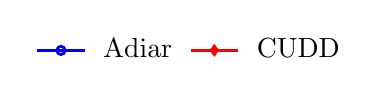
\begin{tikzpicture}
      \begin{customlegend}[
        legend columns=-1,
        legend style={draw=none,column sep=1ex},
        legend entries={Adiar, CUDD}
        ]
        \addlegendimage{style=plot_adiar}
        \addlegendimage{style=plot_cudd}
      \end{customlegend}
    \end{tikzpicture}

    \caption{Running time for \emph{3D Tic-Tac-Toe} with $300$~GiB of RAM.}
  \end{figure}
\end{frame}

\blankframe

\begin{frame}
  \begin{figure}
    \centering
    \Large

    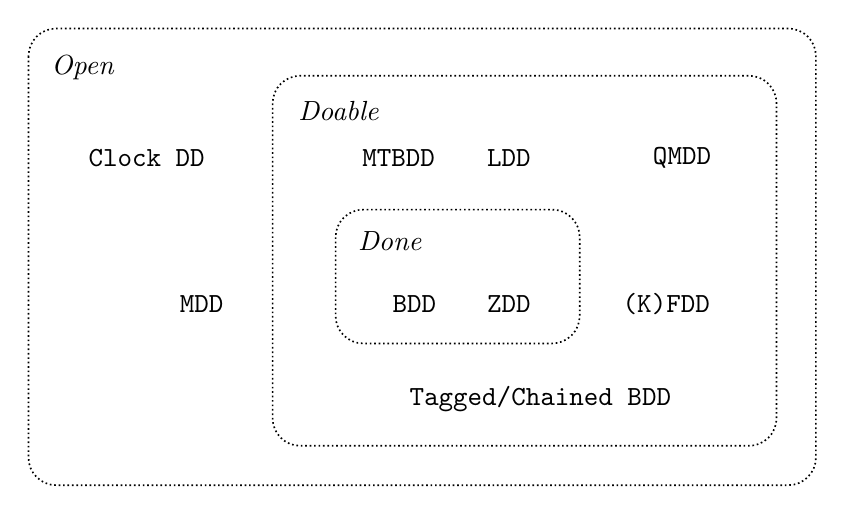
\begin{tikzpicture}
      % Done
      \draw[draw=black, rounded corners=10pt, densely dotted, line width = 0.6pt]
        (-0.5,0.5) rectangle ++(3.1,-1.7);

      \node at (0.2,0.1)  {\emph{Done}};

      \node at (0.5,-0.7) {\texttt{BDD}};
      \node at (1.7,-0.7) {\texttt{ZDD}};

      % Doable
      \onslide<2-> {
        \draw[draw=black, rounded corners=10pt, densely dotted, line width = 0.6pt]
        (-1.3,2.2) rectangle ++(6.4,-4.7);

        \node at (-0.45,1.75)  {\emph{Doable}};

        \node at (3.7,-0.7) {\texttt{(K)FDD}};
        \node at (0.3,1.15) {\texttt{MTBDD}};
        \node at (2.1,-1.9) {\texttt{Tagged/Chained BDD}};
%        \node at (1,-1.6) {\texttt{Tagged BDD}};
%        \node at (0.9,-2.2) {\texttt{Chained BDD}};

        \node at (1.7,1.15) {\texttt{LDD}};

        \node at (3.9,1.15) {\texttt{QMDD}};
      }

      % Open
      \onslide<3-> {
        \draw[draw=black, rounded corners=10pt, densely dotted, line width = 0.6pt]
        (-4.4,2.8) rectangle ++(10,-5.8);

        \node at (-3.7,2.3)  {\emph{Open}};

        \node at (-2.2,-0.7) {\texttt{MDD}};
        \node at (-2.9,1.15) {\texttt{Clock DD}};
      }
    \end{tikzpicture}
  \end{figure}
\end{frame}

\begin{frame}[plain,noframenumbering]
  {\Large \textbf{Steffan Christ Sølvsten}}
  \vspace{1pt} {\hrule width0.45\linewidth}

  \vspace{5pt}

  \begin{itemize}
  \item[\faIcon{envelope}] \mailto{soelvsten@cs.au.dk}
  \item[\faIcon{twitter}] \href{https://www.twitter.com/ssoelvsten}{@ssoelvsten}
  \end{itemize}

  \vspace{10pt}

  {\Large \textbf{Adiar}}
  \vspace{1pt} {\hrule width0.45\linewidth}

  \vspace{5pt}

  \begin{itemize}
  \item[\faIcon{code}]
    \href{http://github.com/ssoelvsten/adiar}{github.com/ssoelvsten/adiar}
  \item[\faIcon{book}\hspace{2pt}]
    \href{http://ssoelvsten.github.io/adiar}{ssoelvsten.github.io/adiar}
  \end{itemize}


  \vspace{10pt}

  
\includegraphics[width=0.2\linewidth]{external/aulogo_uk_var2_black.eps}
\end{frame}

\begin{frame}
  \begin{figure}
    \centering

    \setvalue{timeline_c0 = black}
    \setvalue{timeline_c1 = black}
    \setvalue{timeline_c2 = black}

    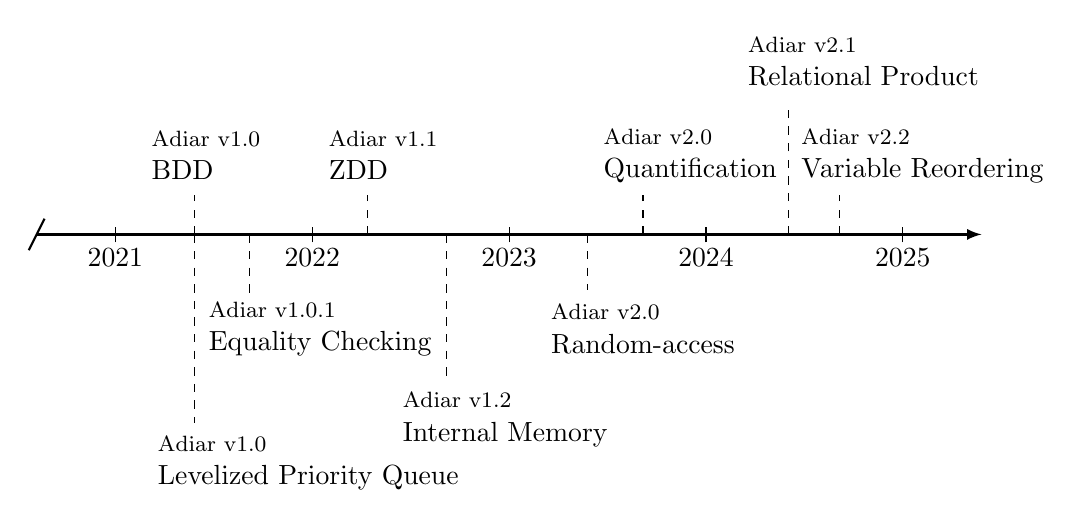
\begin{tikzpicture}
      % Primary line
\draw[-latex, thick] (0,0) -- (12,0);
\draw[thick] (0.1,0.2) -- (-0.1,-0.2);

% 2021
\draw (1,-0.1) -- ++(0,0.2);
\node at (1,-0.3) {$2021$};

\draw[dashed, color=black] (2,0) -- ++(0,0.5);
\node[color=black, align=left] at (2.15,1.0)
{\footnotesize Adiar v1.0\\BDD};

\draw[dashed, color=black] (2,0) -- ++(0,-2.4);
\node[color=black, align=left] at (3.45,-2.9)
{\footnotesize Adiar v1.0\\Levelized Priority Queue};

\draw[dashed, color=black] (2.7,0) -- ++(0,-0.8);
\node[color=black, align=left] at (3.6,-1.2)
{\footnotesize Adiar v1.0.1\\Equality Checking};

% 2022
\draw (3.5,-0.1) -- ++(0,0.2);
\node at (3.5,-0.3) {$2022$};

\draw[dashed, color=black] (4.2,0) -- ++(0,0.5);
\node[color=black, align=left] at (4.4,1.0)
{\footnotesize Adiar v1.1\\ZDD};

\draw[dashed, color=black] (5.2,0) -- ++(0,-1.8);
\node[color=black, align=left] at (5.95,-2.35)
{\footnotesize Adiar v1.2\\Internal Memory};

% 2023
\draw (6,-0.1) -- ++(0,0.2);
\node at (6,-0.3) {$2023$};

\draw[dashed, color=black] (7,0) -- ++(0,-0.7);
\node[color=black, align=left] at (7.7,-1.2)
{\footnotesize Adiar v2.0\\Random-access};

\draw[dashed, color=black] (7.7,0) -- ++(0,0.5);
\node[color=black, align=left] at (8.3,1.0)
{\footnotesize Adiar v2.0\\Quantification};

% 2024
\draw (8.5,-0.1) -- ++(0,0.2);
\node at (8.5,-0.3) (y2024) {$2024$};

\draw[dashed, color=black] (9.55,0) -- ++(0,1.6);
\node[color=black, align=left] at (10.5,2.2)
{\footnotesize Adiar v2.1\\Relational Product};

\draw[dashed, color=black] (10.2,0) -- ++(0,0.5);
\node[color=black, align=left] at (11.25,1.0)
{\footnotesize Adiar v2.2\\Variable Reordering};

% 2025
\draw (11,-0.1) -- ++(0,0.2);
\node at (11,-0.3) (y2025) {$2025$};
    \end{tikzpicture}
  \end{figure}
\end{frame}

\begin{frame}
  \begin{columns}
  \begin{column}{0.49\textwidth}

    \begin{figure}
      \centering

      \begin{subfigure}{1\linewidth}
        \centering

        \begin{tikzpicture}[scale=0.9, every node/.style={transform shape}]
          % nodes
          \node[shape = circle, draw = black]
          (0) {\tiny $(0,0)$};

          \node[shape = circle, draw = black, below right= .3cm and .5cm of 0]
          (1) {\tiny $(1,0)$};

          \node[shape = circle, draw = black, below left=.3cm and .5cm of 1]
          (2) {\tiny $(2,0)$};

          \node[shape = circle, draw = black, below left=.3cm and .5cm of 2]
          (31) {\tiny $(3,0)$};
          \node[shape = circle, draw = black, below right=.3cm and .5cm of 2]
          (32) {\tiny $(3,1)$};

          % leafs
          \node[shape = rectangle, draw = black, below=.4cm of 31]
          (sink_T) {$\top$};

          \node[shape = rectangle, draw = black, below=.4cm of 32]
          (sink_F) {$\bot$};

          % arcs
          \draw[->,dashed]
          (0) edge (2)
          (1) edge (2)
          (2) edge (31)
          (31) edge (sink_T)
          (32) edge (sink_F)
          ;

          \draw[->]
          (0) edge (1)
          (1) edge (32)
          (2) edge (32)
          (31) edge (sink_F)
          (32) edge (sink_T)
          ;

          % animations
          \onslide<3-5>{ % 0
            \node[shape = circle, orange, draw = orange]
            {\tiny $(0,0)$};
            \draw[->,dashed,orange] (0) edge (2);
            \draw[->,orange] (0) edge (1);
          }

          \onslide<6-9>{ % 1
            \node[shape = circle, orange, draw = orange, below right= .3cm and .5cm of 0]
            {\tiny $(1,0)$};
            \draw[->,dashed,orange] (1) edge (2);
            \draw[->,orange] (1) edge (32);
          }

          \onslide<10-14>{ % 2
            \node[shape = circle, orange, draw = orange, below left=.3cm and .5cm of 1]
            {\tiny $(2,0)$};
            \draw[->,dashed,orange] (2) edge (31);
            \draw[->,orange] (2) edge (32);
          }

          \onslide<15-18>{ % 31
            \node[shape = circle, orange, draw = orange, below left=.3cm and .5cm of 2]
            {\tiny $(3,0)$};
            \draw[->,dashed,orange] (31) edge (sink_T);
            \draw[->,orange] (31) edge (sink_F);
          }

          \onslide<19-22>{ % 32
            \node[shape = circle, orange, draw = orange, below right=.3cm and .5cm of 2]
            {\tiny $(3,1)$};
            \draw[->,dashed,orange] (32) edge (sink_F);
            \draw[->,orange] (32) edge (sink_T);
          }
        \end{tikzpicture}

        \caption{\small $(x_0 \wedge x_1 \wedge x_3) \vee (x_2 \oplus x_3)$}
      \end{subfigure}

      %\caption{In-order traversal of BDD}
    \end{figure}

  \end{column}
  \begin{column}{0.49\textwidth}
    \centering

    \onslide<5->{ \small
      \begin{tabular}{c c c}
        \onslide<5-22>{\hspace{10pt}Seek\hspace{10pt}}
        \onslide<5-22>{& \hspace{10pt}Sum\hspace{10pt}}
        \onslide<5-23>{& \hspace{10pt}Result\hspace{10pt}}
        \\
        \textcolor{orange}{%
        \only<5-8>{$(1,0)$}%
        \only<9-13>{$(2,0)$}%
        \only<14-17>{$(3,0)$}%
        \only<18-22>{$(3,1)$}%
        }
        &
        % (1,0)
          \only<5-6>{$0$}%
          \only<7-8>{$1$}%
          % (2,0)
          \only<9-10>{$0$}%
          \only<11>{$1$}%
          \only<12-13>{$2$}%
          % (3,0)
          \only<14-15>{$0$}%
          \only<16-17>{$2$}%
          % (3,1)
          \only<18-19>{$0$}%
          \only<20>{$1$}%
          \only<21-22>{$3$}%
        &
          \only<1-16>{$0$}%
          \only<17-21>{$2$}%
          \only<22-23>{$5$}%
      \end{tabular}
    }

    \vspace{20pt}

    \onslide<2->{
      {\footnotesize Priority Queue: $Q_{\mathit{count}}$:

        \begin{tabular}{rll}
          [ & \onslide<4-6>{$(\arc{(0,0)}{\top}{(1,0)}, \quad 1)$  & ,}
          \\
            & \onslide<4-10>{$(\arc{(0,0)}{\bot}{(2,0)}, \quad 1)$  & ,}
          \\
            & \onslide<8-11>{$(\arc{(1,0)}{\bot}{(2,0)}, \quad 1)$  & ,}
          \\
            & \onslide<13-15>{$(\arc{(2,0)}{\bot}{(3,0)}, \quad 2)$  & ,}
          \\
            & \onslide<8-19>{$(\arc{(1,0)}{\top}{(3,1)}, \quad 1)$   & ,}
          \\
            & \onslide<13-20>{$(\arc{(2,0)}{\top}{(3,1)}, \quad 2)$ }  & ]
        \end{tabular}
      }
    }

  \end{column}
\end{columns}

\end{frame}

\begin{frame}[plain,noframenumbering]
  {\Large \textbf{Steffan Christ Sølvsten}}
  \vspace{1pt} {\hrule width0.45\linewidth}

  \vspace{5pt}

  \begin{itemize}
  \item[\faIcon{envelope}] \mailto{soelvsten@cs.au.dk}
  \item[\faIcon{twitter}] \href{https://www.twitter.com/ssoelvsten}{@ssoelvsten}
  \end{itemize}

  \vspace{10pt}

  {\Large \textbf{Adiar}}
  \vspace{1pt} {\hrule width0.45\linewidth}

  \vspace{5pt}

  \begin{itemize}
  \item[\faIcon{code}]
    \href{http://github.com/ssoelvsten/adiar}{github.com/ssoelvsten/adiar}
  \item[\faIcon{book}\hspace{2pt}]
    \href{http://ssoelvsten.github.io/adiar}{ssoelvsten.github.io/adiar}
  \end{itemize}


  \vspace{10pt}

  
\includegraphics[width=0.2\linewidth]{external/aulogo_uk_var2_black.eps}
\end{frame}


\end{document}

%%% Local Variables:
%%% mode: latex
%%% TeX-master: t
%%% End:
